\documentclass[11pt]{article}

\usepackage[letterpaper,margin=0.75in]{geometry}
\usepackage{booktabs}
\usepackage{graphicx}
\usepackage{listings}
\usepackage{hyperref}

\setlength{\parindent}{1.4em}

\begin{document}

\lstset{
  language=Python,
  basicstyle=\small,          % print whole listing small
  keywordstyle=\bfseries,
  identifierstyle=,           % nothing happens
  commentstyle=,              % white comments
  stringstyle=\ttfamily,      % typewriter type for strings
  showstringspaces=false,     % no special string spaces
  numbers=left,
  numberstyle=\tiny,
  numbersep=5pt,
  frame=tb,
}

\newenvironment{absolutelynopagebreak}
  {\par\nobreak\vfil\penalty0\vfilneg
   \vtop\bgroup}
  {\par\xdef\tpd{\the\prevdepth}\egroup
   \prevdepth=\tpd}

\title{Network Simulation}

\author{Cody Heffner}

\date{19 Mar. 2015}

\maketitle

\section{Preface}

This report details the experiment I ran and the results obtained as specified by the Congestion Control Lab in the BYU CS 460 class taught by Dr. Zappala. The project specifications can be found \href{http://cs460.byu.edu/winter-2015/labs/congestion-control-part-2}{here}.

The experiment requires heavy use of a network simulator to test different network scenarios. The network simulator I used is Dr. Zappala's \href{https://github.com/zappala/bene}{Bene}, written in Python. All my simulation examples shown will be tailored towards use for that simulator.

\section{Summary}

The goal of this lab was to implement congestion control in my implementation of TCP. This includes implementing TCP slow start and TCP additive increase, multiplicative decrease, as well as a fast-retransmit function. This portion of the lab specifically tests congestion when there is more than one flow incoming to the same node.

In every experiment other than the final one (\emph{Advanced Experiment: Competing Round Trip Time}), I created a network consisting of two nodes and one bi-directional link with a link bandwidth of 10 Mbps, 10 ms propagation delay, and a queue size of 100 packets (100,000 bytes). The test file was of size 1 MB.


% ##########################################################


\section{Basic Experiment: One Flow}

This experiment's purpose was to establish a base case and teach us what a single flow looks like. The following three figures respectively show the sequence graph, a graph of the receiver's rate over time during the download, and a scatter plot of the queue during the download.

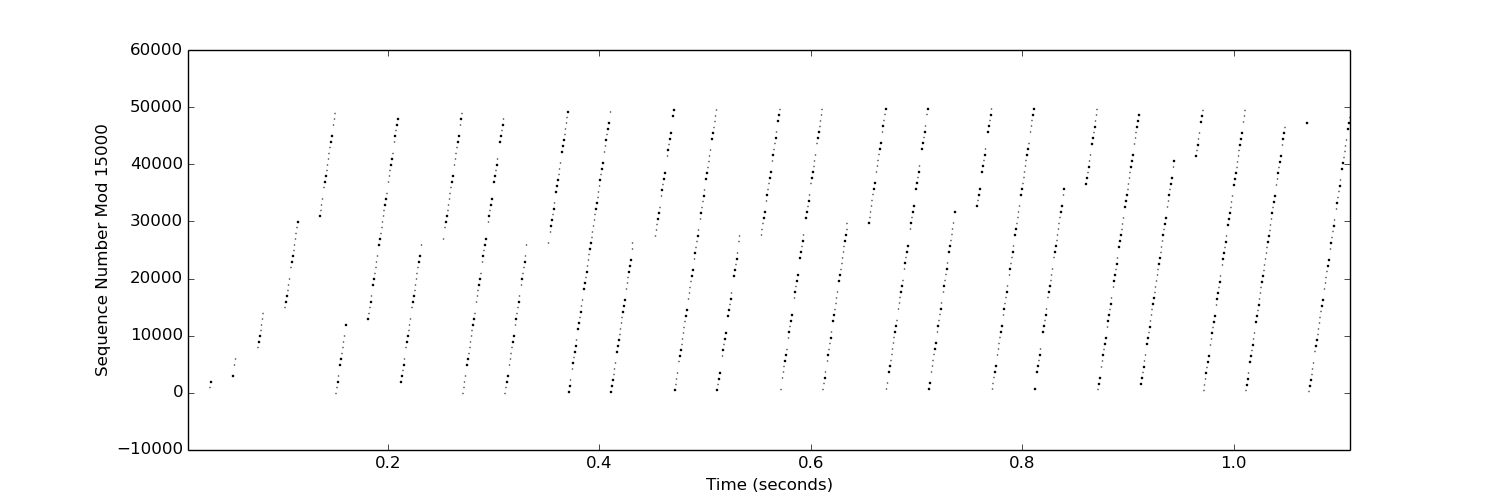
\includegraphics[width=17cm]{outputs/oneflow/oneflow_sequence.png}

\centerline{\emph{Figure 1.1: Sequence Graph of One Flow}}

This graph shows the standard send-ACK relationship as the file is transferred.


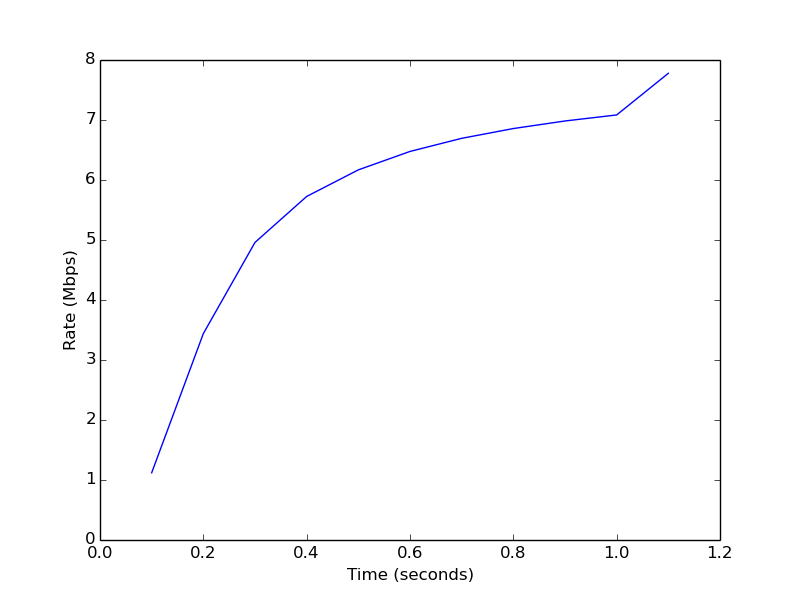
\includegraphics[width=17cm]{outputs/oneflow/oneflow_rate.png}

\centerline{\emph{Figure 1.2: Rate Graph of One Flow}}

The rate is a smooth curve when the file transfer starts in slow-start mode. When it reaches its threshold, when TCP congestion control transfers into additive increase, the rate increases linearly until the file transfer completes.


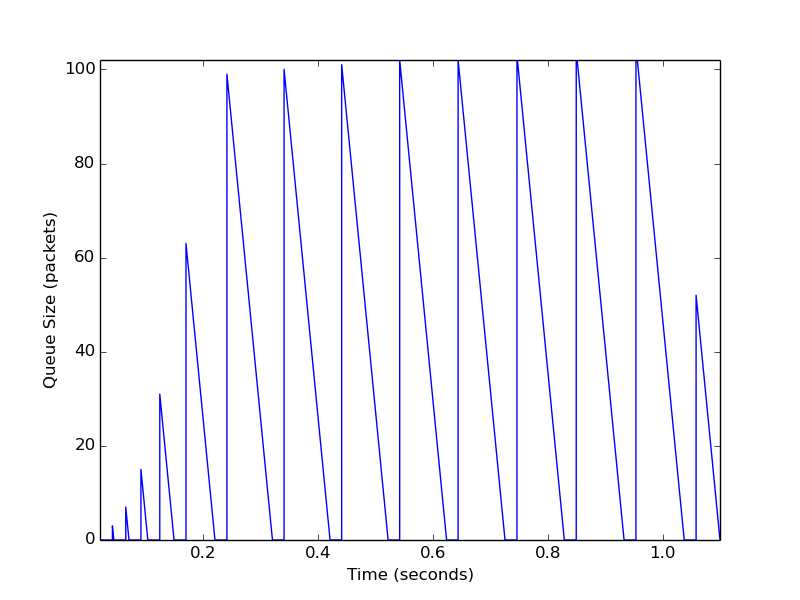
\includegraphics[width=17cm]{outputs/oneflow/oneflow_queue.png}

\centerline{\emph{Figure 1.3: Queue Graph of One Flow}}

The queue for the first node steadily increases until it reaches its maximum, then quickly decreases as the file transfer completes.


% ##########################################################


\section{Basic Experiment: Two Flows}

This experiment's purpose was to introduce multiple flows while keeping it as simple as possible. Both flows begin at time \emph{t=0s}. The following four figures respectively show the sequence graph for each flow, a graph of the receiver's rates over time during the download, and a scatter plot of the sender's queue during the download.

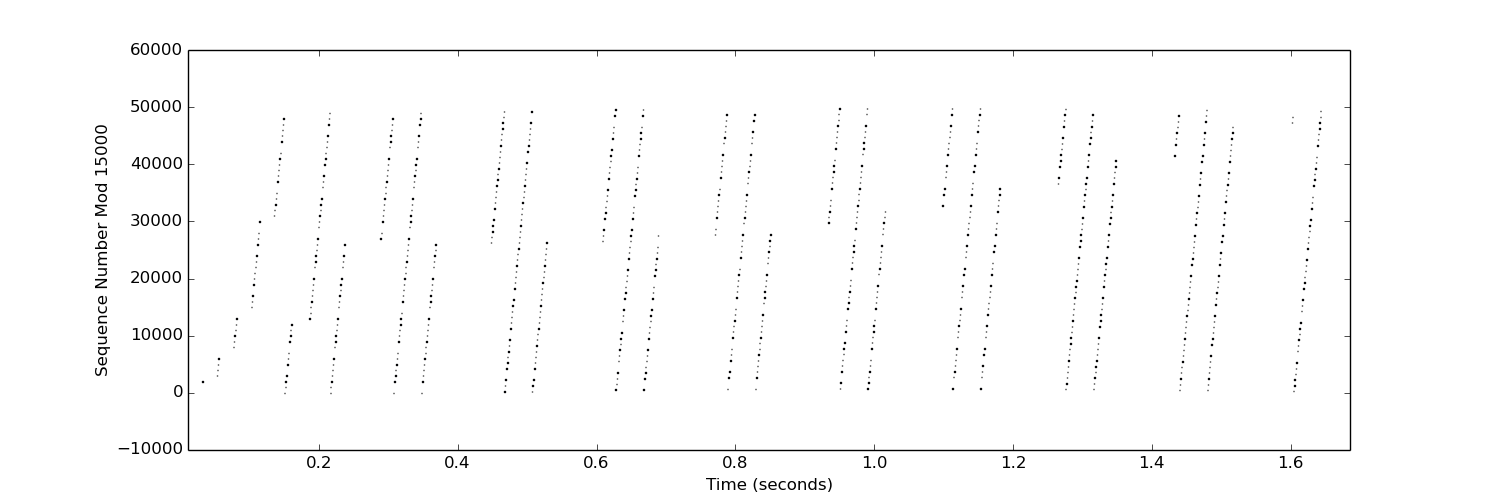
\includegraphics[width=17cm]{outputs/twoflows/twoflows_sequence1.png}

\centerline{\emph{Figure 2.1a: Sequence Graph of the First of Two Flows}}

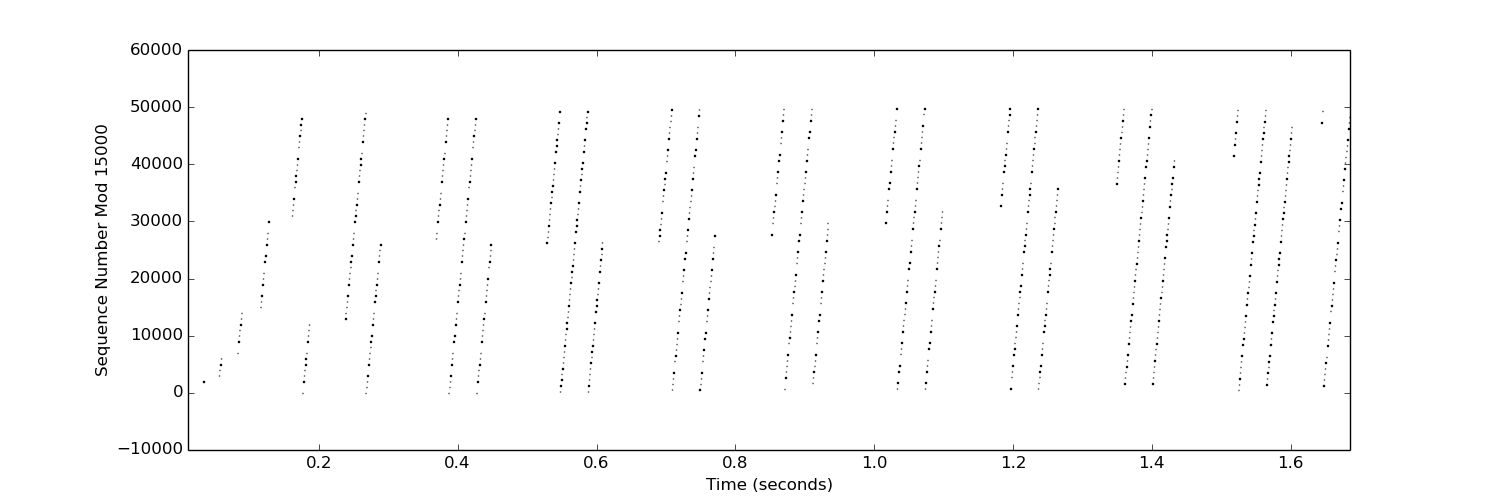
\includegraphics[width=17cm]{outputs/twoflows/twoflows_sequence2000.png}

\centerline{\emph{Figure 2.1b: Sequence Graph of the Second of Two Flows}}

Both flows appear to be quite evenly spaced (compare with figures 3.1a-3.1e), indicating that bandwidth is nearly evenly shared as the file transfers.


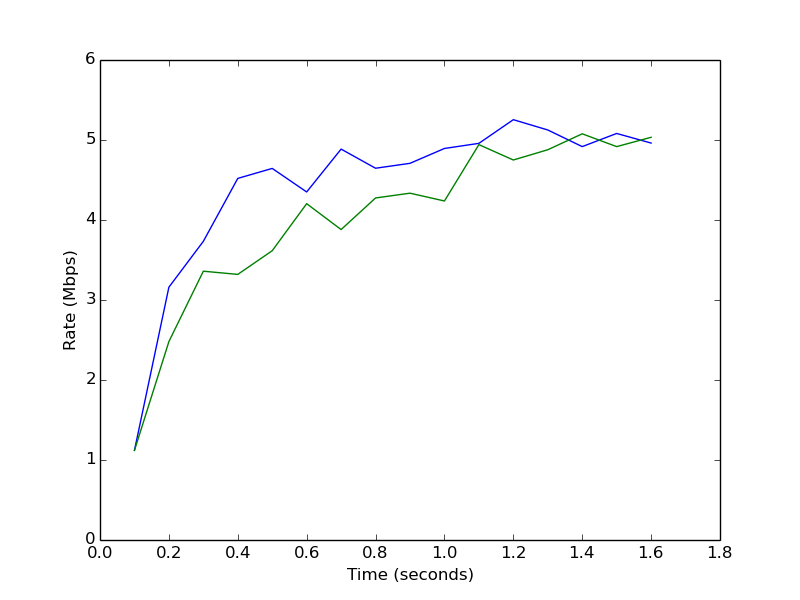
\includegraphics[width=17cm]{outputs/twoflows/twoflows_rate.png}

\centerline{\emph{Figure 2.2: Rate Graph of Two Flows}}

This graph confirms the previous theory that bandwidth is nearly evenly shared. As the file transfer rates combined approach the maximum rate the line can physically support (10 Mbps), they realize that they are using the maximum capability of the line and begin to balance out around 5 Mbps each. I hypothesize that the graphs would continue on in their braided fashion if the file was larger.


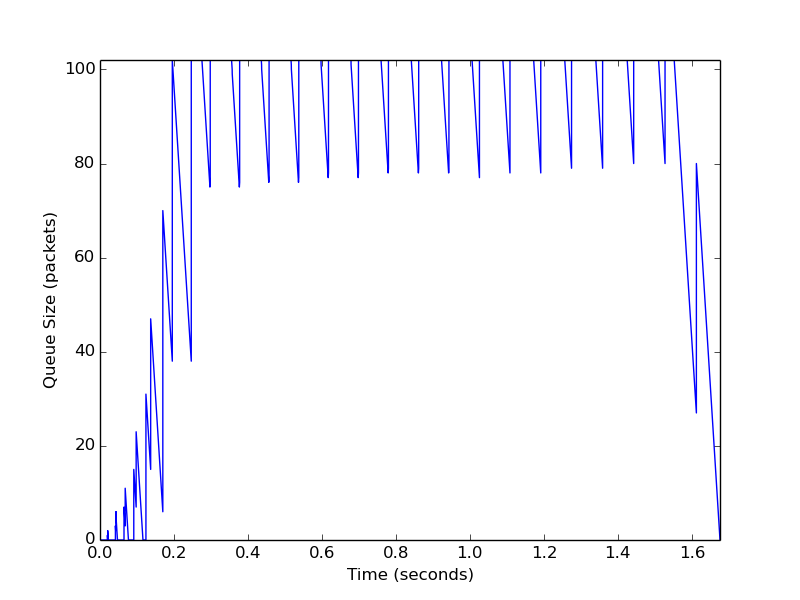
\includegraphics[width=17cm]{outputs/twoflows/twoflows_queue.png}

\centerline{\emph{Figure 2.3: Queue Graph of Two Flows}}

The size of the queue rapidly approaches its maximum capacity, since twice as many bytes are attempting to be transferred per send+ACK round.


% ##########################################################


\section{Basic Experiment: Five Flows}

This experiment's purpose was to induce stress on the link, and thus, on the TCP congestion control algorithm. The first flow begins at time \emph{t=0s}, and each flow begins \emph{0.1s} after the previous flow. The following seven figures respectively show the sequence graph for each flow, a graph of the receiver's rates over time during the download, and a scatter plot of the sender's queue during the download.

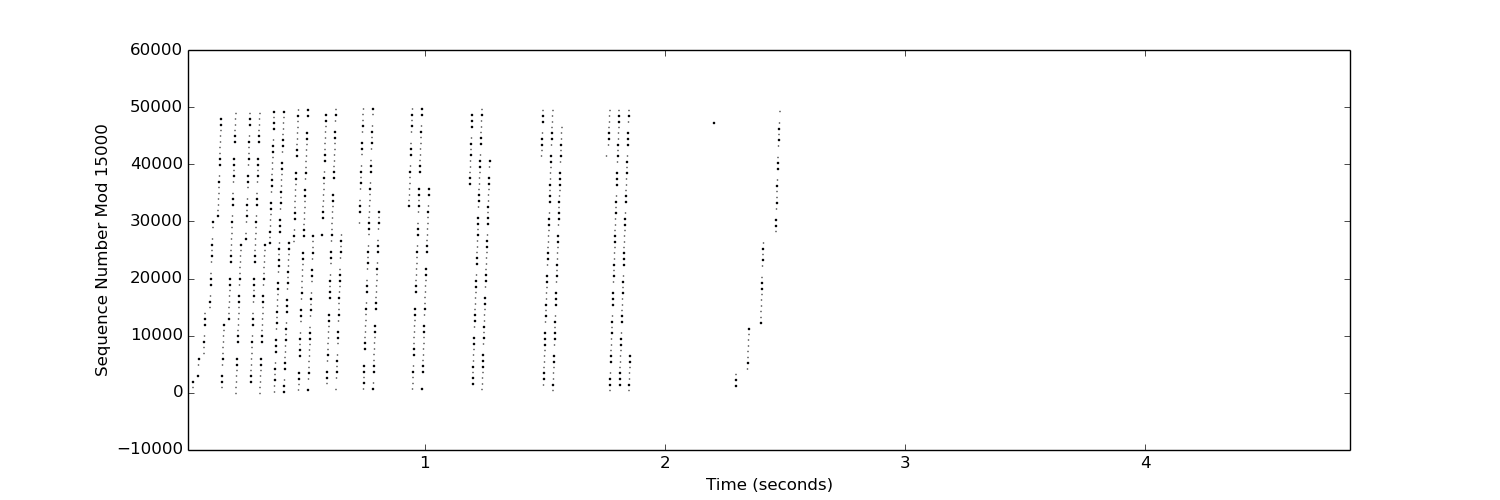
\includegraphics[width=17cm]{outputs/fiveflows/fiveflows_sequence1000.png}

\centerline{\emph{Figure 3.1a: Sequence Graph of the First of Five Flows}}

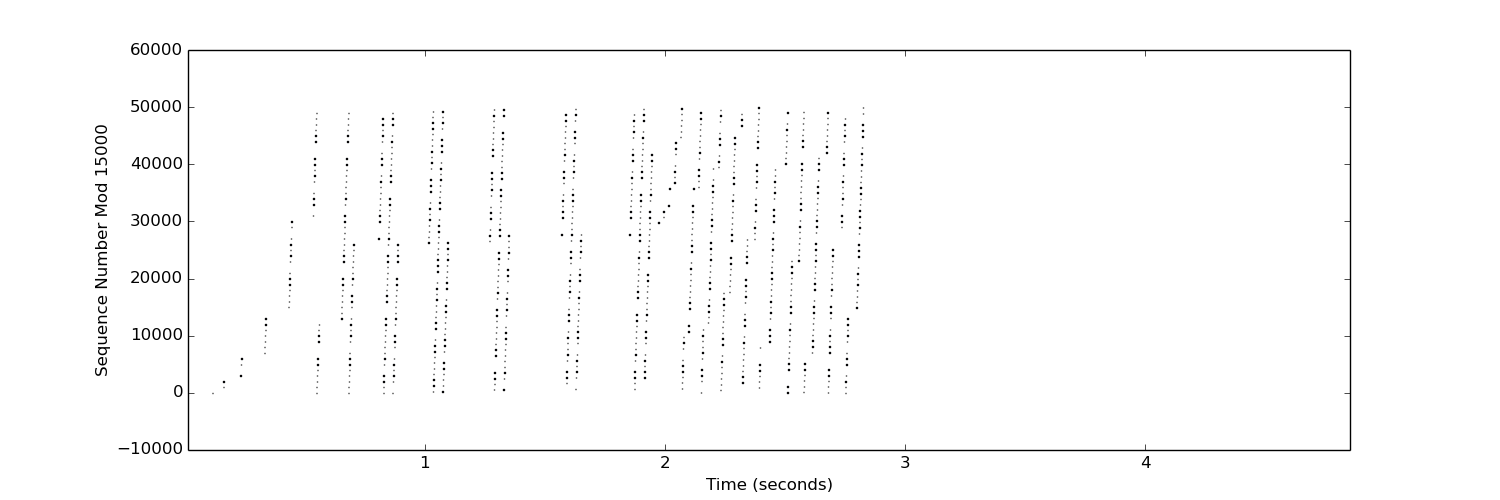
\includegraphics[width=17cm]{outputs/fiveflows/fiveflows_sequence2000.png}

\centerline{\emph{Figure 3.1b: Sequence Graph of the Second of Five Flows}}

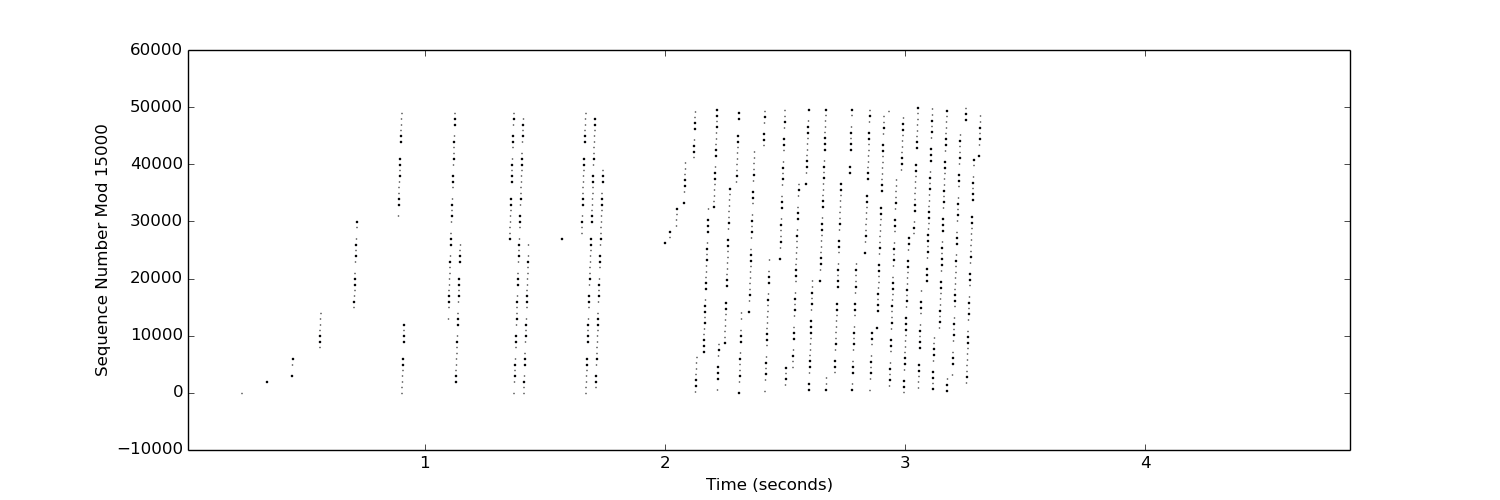
\includegraphics[width=17cm]{outputs/fiveflows/fiveflows_sequence3000.png}

\centerline{\emph{Figure 3.1c: Sequence Graph of the Third of Five Flows}}

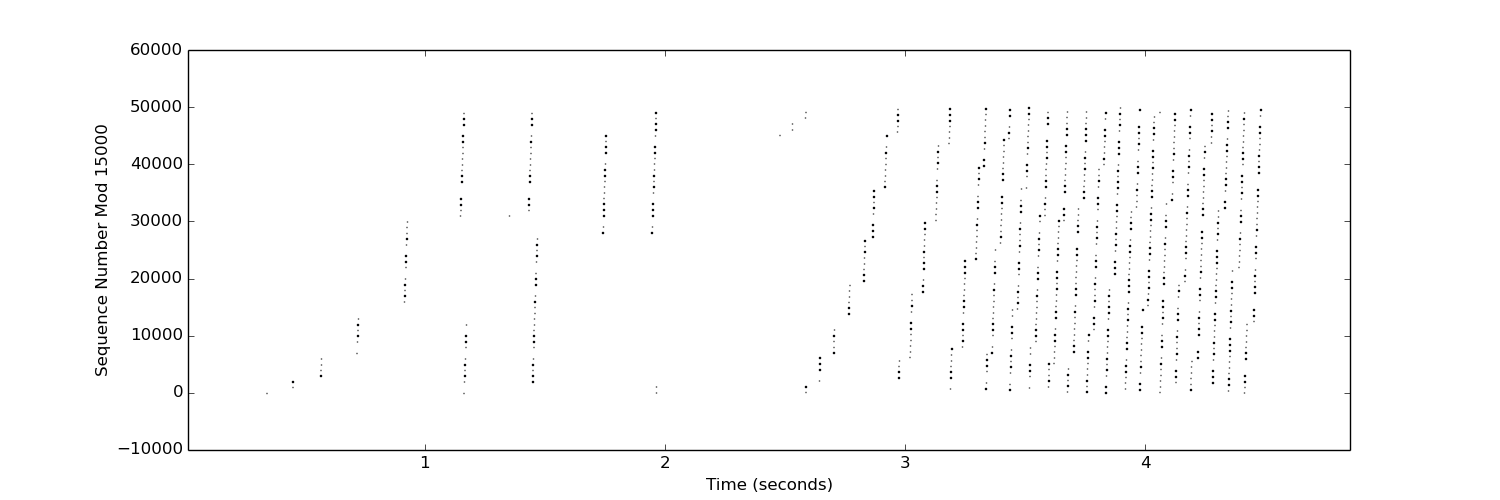
\includegraphics[width=17cm]{outputs/fiveflows/fiveflows_sequence4000.png}

\centerline{\emph{Figure 3.1d: Sequence Graph of the Fourth of Five Flows}}

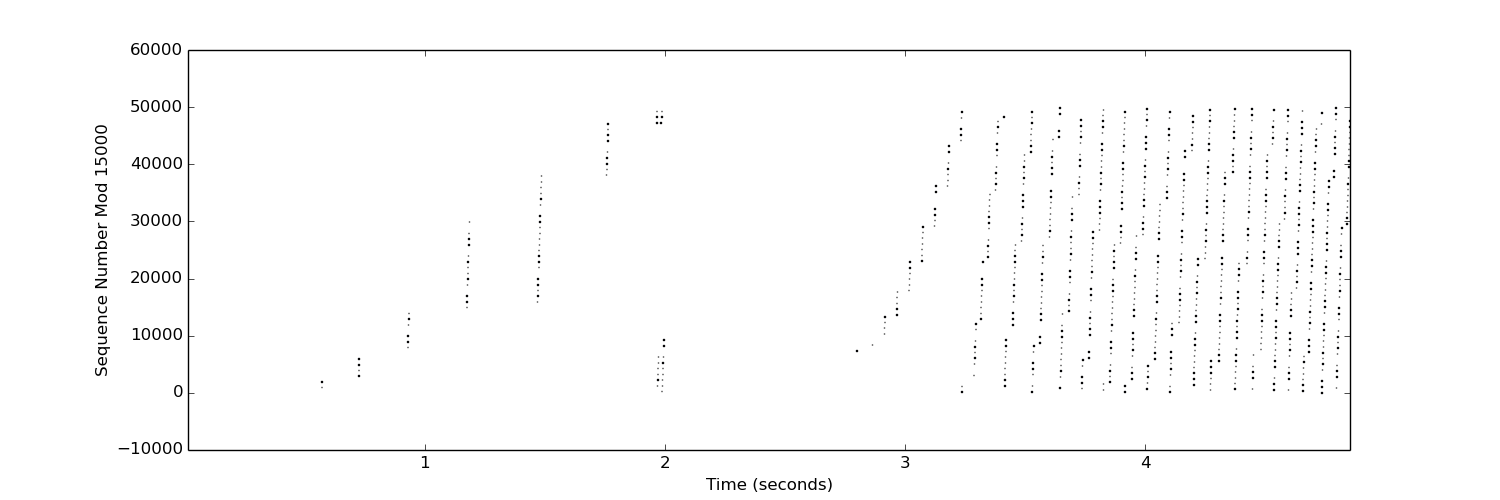
\includegraphics[width=17cm]{outputs/fiveflows/fiveflows_sequence5000.png}

\centerline{\emph{Figure 3.1e: Sequence Graph of the Fifth of Five Flows}}

Unlike the sequence plots of two flows (figures 2.1a-2.1b), the five flow sequence plots show that the flows are \emph{not} evenly spaced. This indicates that some flows utilized the link more than others at certain times. For example, the first file transfer (figure 3.1a) got a large amount of data transferred before the others really had time to get going, while the last two file transfers (figures 3.1d and 3.1e) had to compete together after \emph{t=3s}.


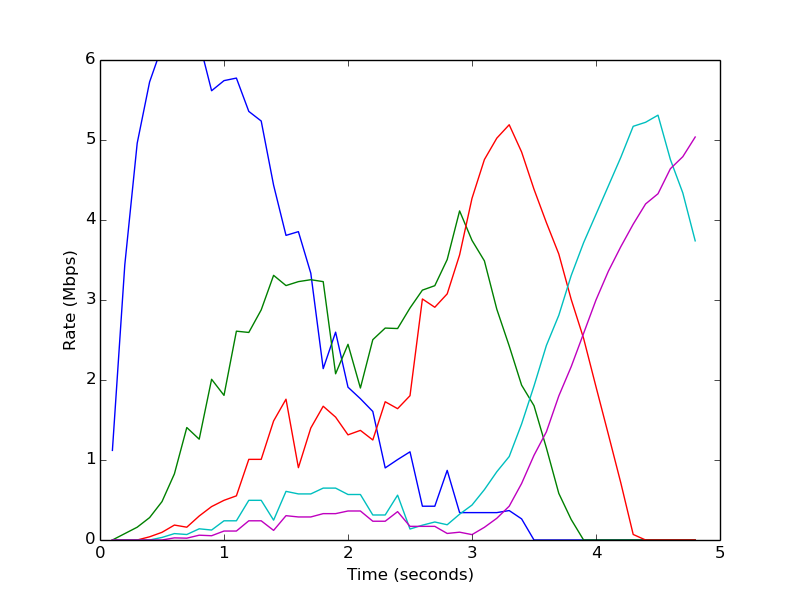
\includegraphics[width=17cm]{outputs/fiveflows/fiveflows_rate.png}

\centerline{\emph{Figure 2.2: Rate Graph of Two Flows}}

This graph confirms the previous theory that bandwidth is not evenly shared. The first flow didn't purposely use more resources than the others; it was simply a result of staggering the start of the flows. TCP slow start let each flow continue in additive increase until a loss event, so the first flow got an entire half-second head start on the fifth flow. By the time a loss event occurred, the first flow looks to be nearly a third of the way done with its transfer (total bytes transferred is the integral of the rate, or the area under each curve). 

Since the link can support up to 10 Mbps transfer speed, the sum of the area under all curves after the first loss event and before all files have finished transferring at any specific point in time should be close to 10 Mbps. For example, at \emph{t=1s}, the sum of the red, cyan, and purple values look to be approximately 1 Mbps, green is at approximately 2 Mbps, and blue is at approximately 6 Mbps. This indicates that at that point in time, the total rate is approximately 9 Mbps.


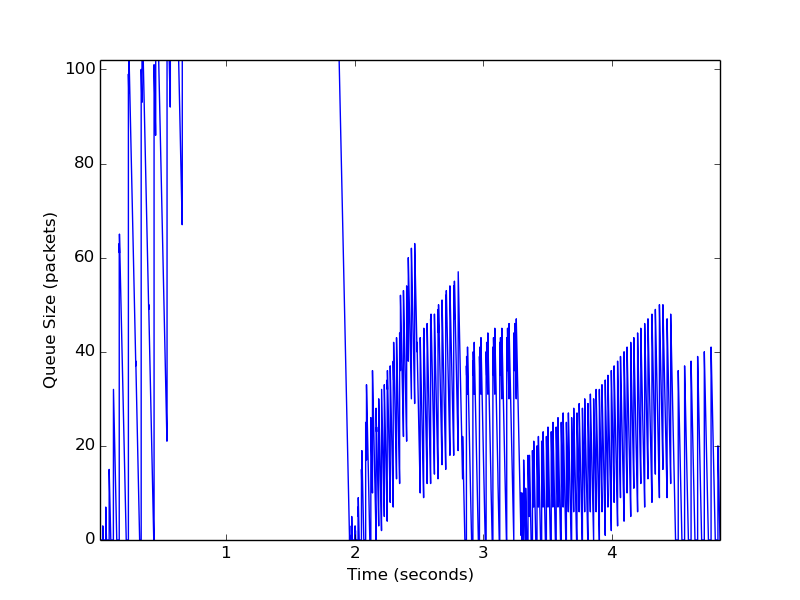
\includegraphics[width=17cm]{outputs/fiveflows/fiveflows_queue.png}

\centerline{\emph{Figure 2.3: Queue Graph of Two Flows}}

The size of the queue rapidly approaches its maximum capacity, since five times as many bytes are attempting to be transferred per send+ACK round.


% ##########################################################


\section{Advanced Experiment: Additive Increase Additive Decrease (AIAD)}

This experiment was to compare the behavior of TCP congestion control when using \emph{Additive Decrease} instead of \emph {Multiplicative Decrease}. In normal TCP congestion control, when a loss event occurs, TCP Tahoe resets its current window size to 1; in other words, it only sends one segment at a time. It also halves its threshold so that it will drop out of slow start (exponential increase) sooner. This is extremely useful when a new user needs to share the link. Multiplicative decrease allows all users to converge to the same proportion of the link's maximum bandwidth; if five users are on the link, each user will get 1/5th of the bandwidth. 

If multiplicative decrease is changed instead to additive decrease, new users on a link will need to wait for the previous users to finish whatever they are doing on the link before they can really start using the link. This experiment shows that.

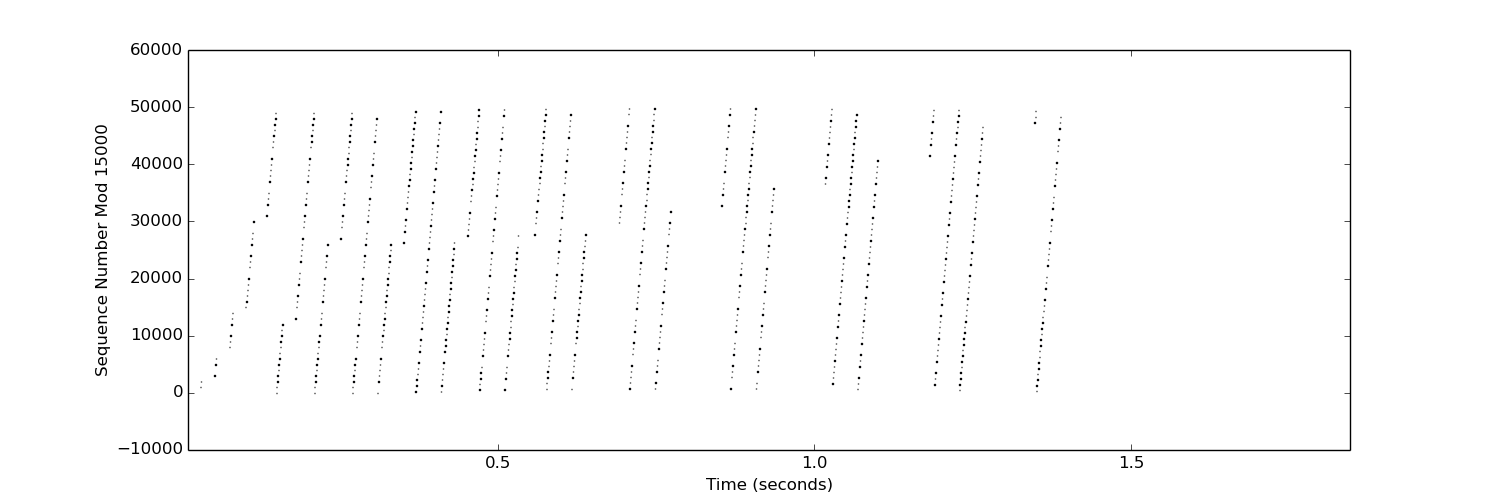
\includegraphics[width=17cm]{outputs/AIAD/AIAD_sequence1000.png}

\centerline{\emph{Figure 4.1a: Sequence Graph of the First of Two Flows in AIAD Mode}}

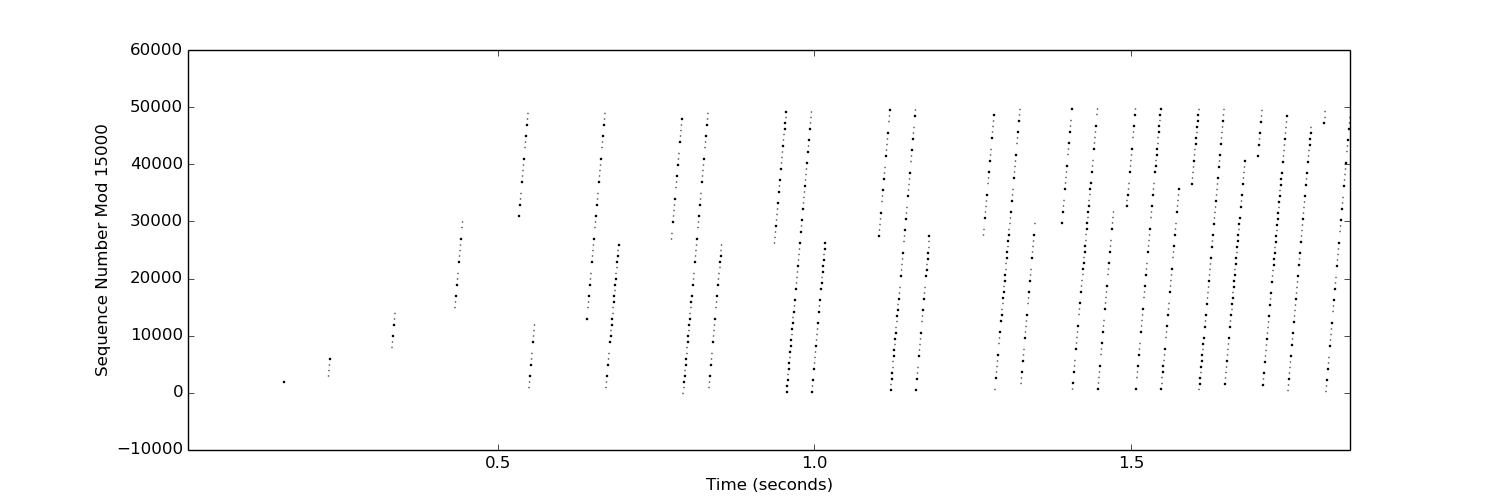
\includegraphics[width=17cm]{outputs/AIAD/AIAD_sequence2000.png}

\centerline{\emph{Figure 4.1b: Sequence Graph of the Second of Two Flows in AIAD Mode}}


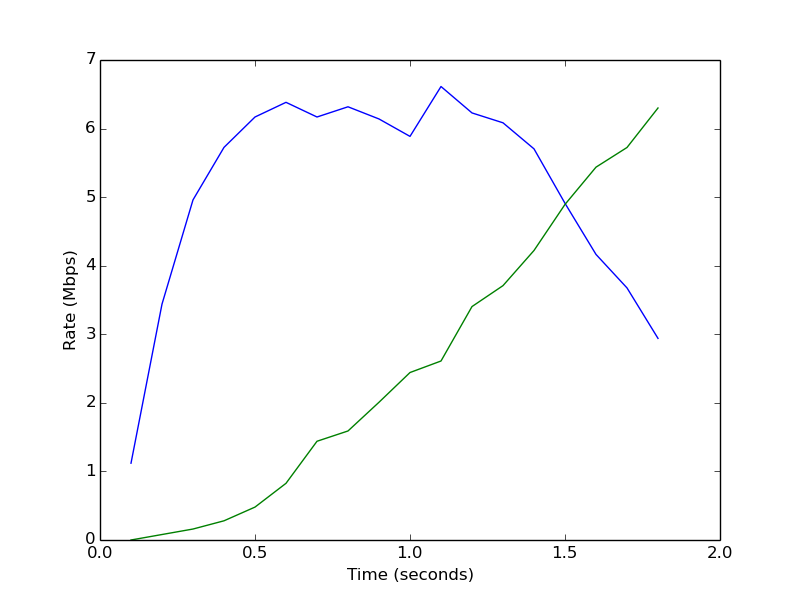
\includegraphics[width=17cm]{outputs/AIAD/AIAD_rate.png}

\centerline{\emph{Figure 4.2: Rate Graph of Two Flows in AIAD Mode}}

The first flow puts a large amount of segments on the line very rapidly, getting a jump start on the second flow. The second flow is increasing where it can, but it isn't allowed to get going until the first flow has completed. 

If the second flow had been delayed even longer, and the first flow had to transfer a file larger than 1 MB, the graph would be even more dismal. The blue line would be extremely close to 10 Mbps and the green line would be stuttering along until the first flow finished.


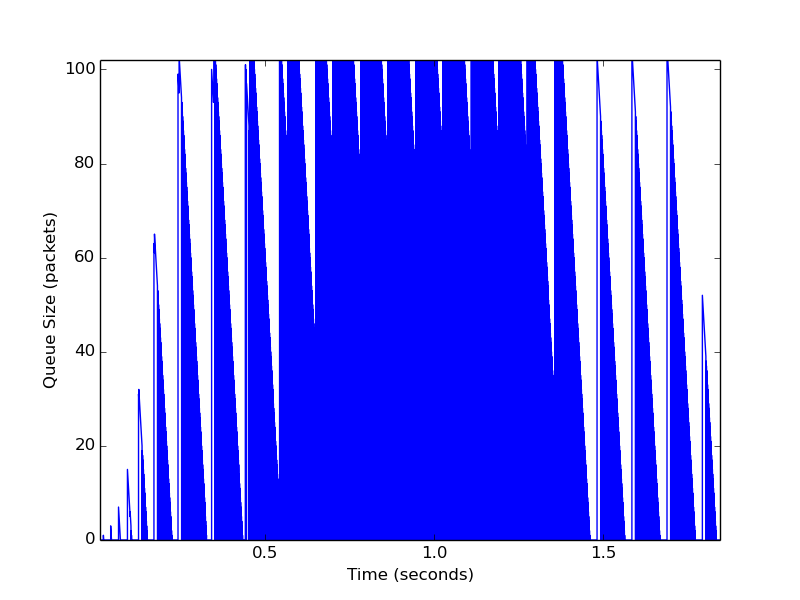
\includegraphics[width=17cm]{outputs/AIAD/AIAD_queue.png}

\centerline{\emph{Figure 4.3: Queue Graph of Two Flows in AIAD Mode.}}

I couldn't figure out why the plotter decided to fill solid colors under the curve, unlike the previous queue graphs. The queue is at max capacity for nearly the entire session.


% ##########################################################


\section{Advanced Experiment: Additive Increase Multiplicative Decrease (AIMD)}

The purpose of this experiment was to compare the specified behavior of TCP congestion control's Multiplicative Decrease with a custom value for multiplicative decreasing. TCP standards state that the threshold is to be halved when a loss event occurs \emph{(threshold = threshold * 1/2)}. This experiment used 5/6th the window size, or \emph{(threshold = threshold * 5/6)}.

In theory, any multiplicative decrease should still allow TCP to function as flows enter and exit the link. The lower the multiplicative value (i.e. the closer to zero), the faster TCP should react to a new flow and allow a new user some portion of the link's bandwidth. However, the lower the value, the lower the utilization of the link during a loss event. The higher the multiplicative value (i.e. the closer to 1), the slower TCP should react and allow a new user some portion of the link's bandwidth, but the higher the utilization of the link during a loss event.

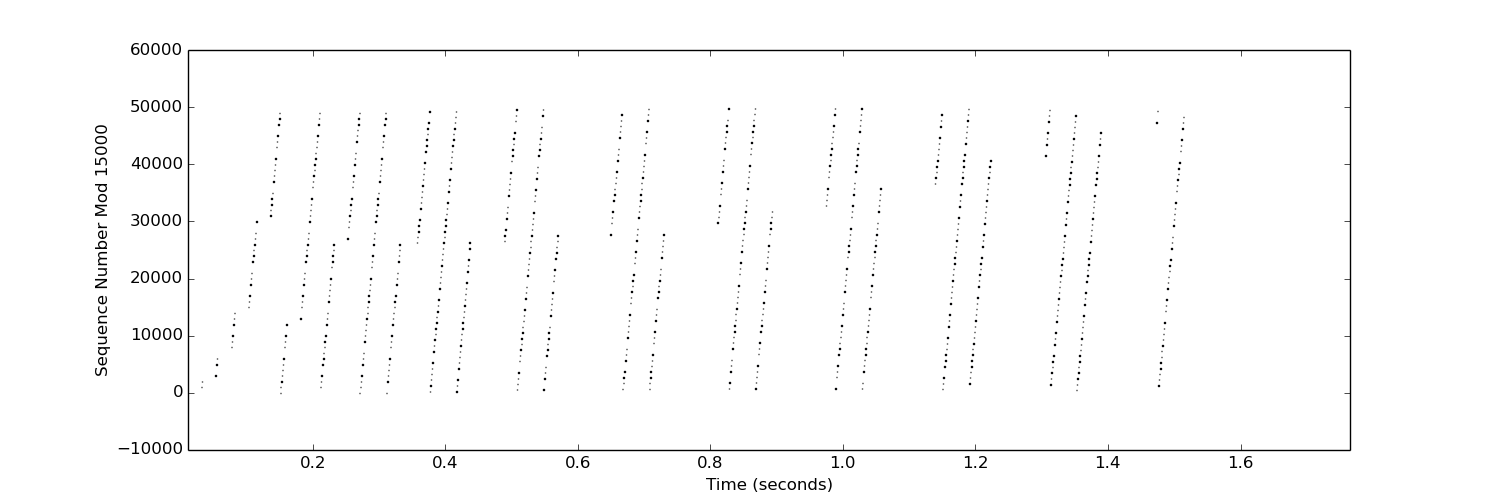
\includegraphics[width=17cm]{outputs/AIMD/AIMD_sequence1000.png}

\centerline{\emph{Figure 5.1a: Sequence Graph of the First of Two Flows in AIMD Mode}}

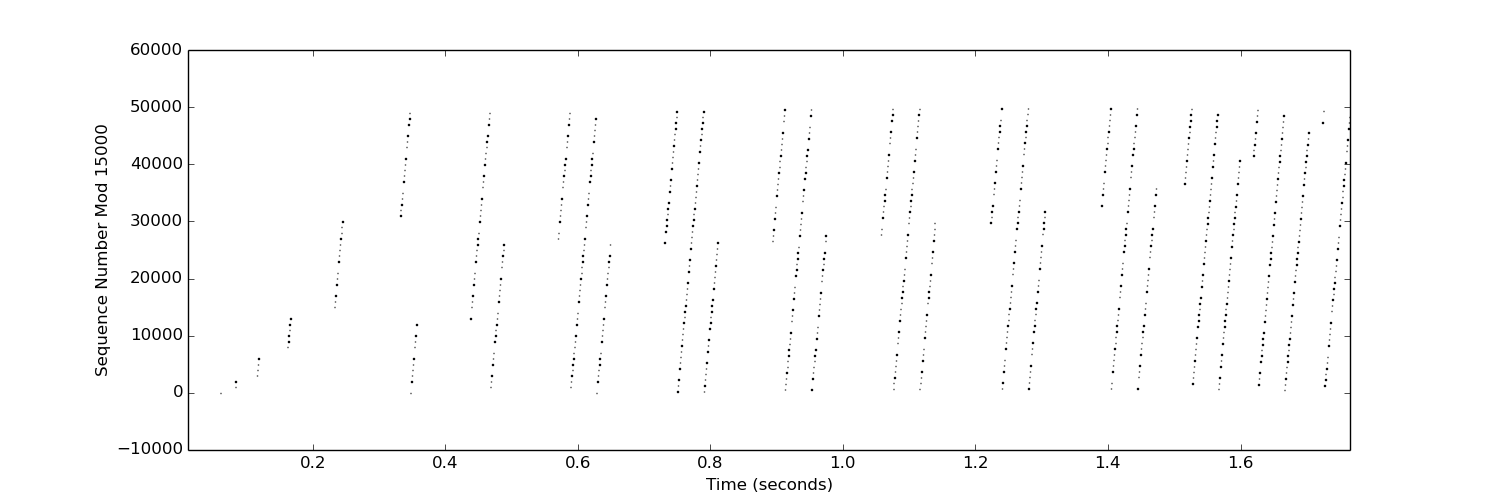
\includegraphics[width=17cm]{outputs/AIMD/AIMD_sequence2000.png}

\centerline{\emph{Figure 5.1b: Sequence Graph of the Second of Two Flows in AIMD Mode}}


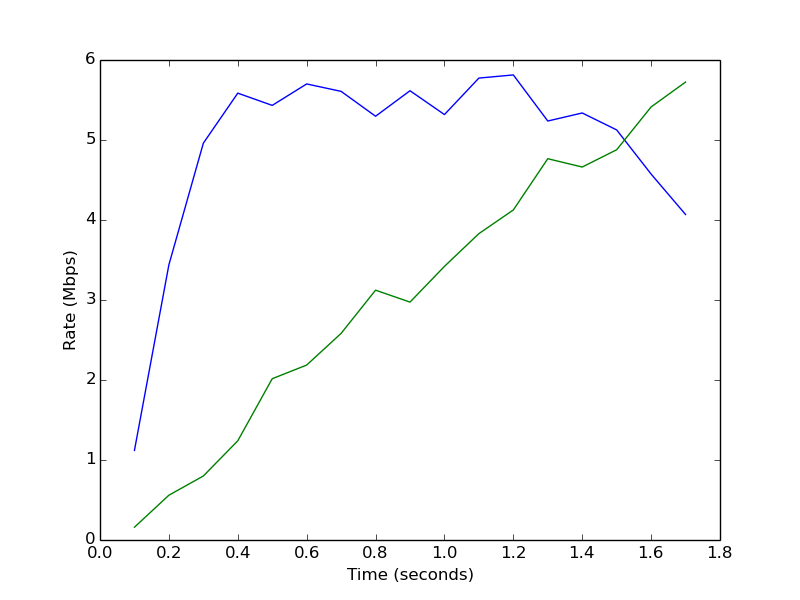
\includegraphics[width=17cm]{outputs/AIMD/AIMD_rate.png}

\centerline{\emph{Figure 5.2: Rate Graph of Two Flows in AIMD Mode}}

The first flow puts a large amount of segments on the line very rapidly, getting a jump start on the second flow. The second flow is increasing where it can, and is allowed a higher portion of the link when compared to AIAD (figure 4.2). 

If the second flow had been delayed even longer, and the first flow had to transfer a file larger than 1 MB, the graph would be more interesting. The blue line would be extremely close to 10 Mbps to start, but as time continued to pass, the blue line would share more and more of the link. If allowed to transfer long enough, they would both eventually reach 5 Mbps transfer speed.


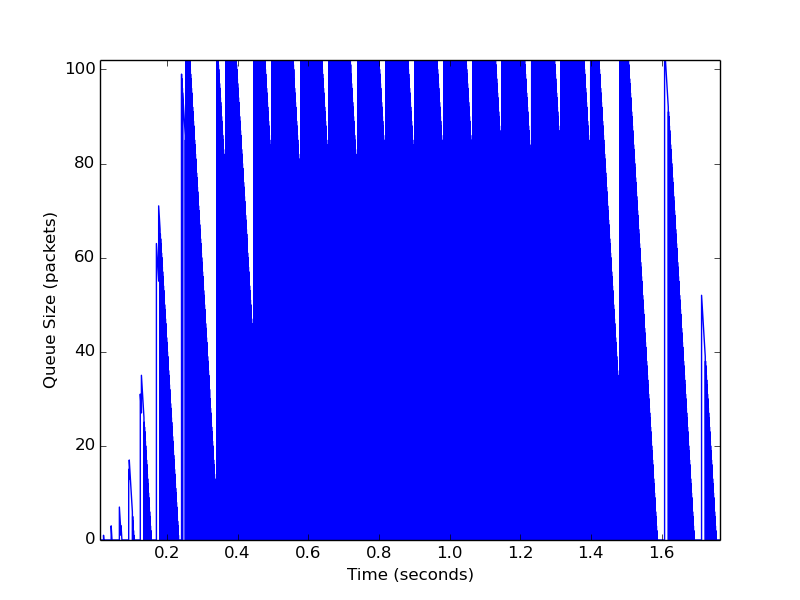
\includegraphics[width=17cm]{outputs/AIMD/AIMD_queue.png}

\centerline{\emph{Figure 5.3: Queue Graph of Two Flows in AIMD Mode.}}

The queue graph again shows that the queue is nearly full for nearly the entire duration.


% ##########################################################


\section{Advanced Experiment: Competing AIMD}

The purpose of this experiment was to compare the specified behavior of TCP congestion control's Multiplicative Decrease with a custom value for multiplicative decreasing. TCP standards state that the threshold is to be halved when a loss event occurs \emph{(threshold = threshold * 1/2)}. This experiment used 5/6th the window size, or \emph{(threshold = threshold * 5/6)}.

In theory, any multiplicative decrease should still allow TCP to function as flows enter and exit the link. The lower the multiplicative value (i.e. the closer to zero), the faster TCP should react to a new flow and allow a new user some portion of the link's bandwidth. However, the lower the value, the lower the utilization of the link during a loss event. The higher the multiplicative value (i.e. the closer to 1), the slower TCP should react and allow a new user some portion of the link's bandwidth, but the higher the utilization of the link during a loss event.

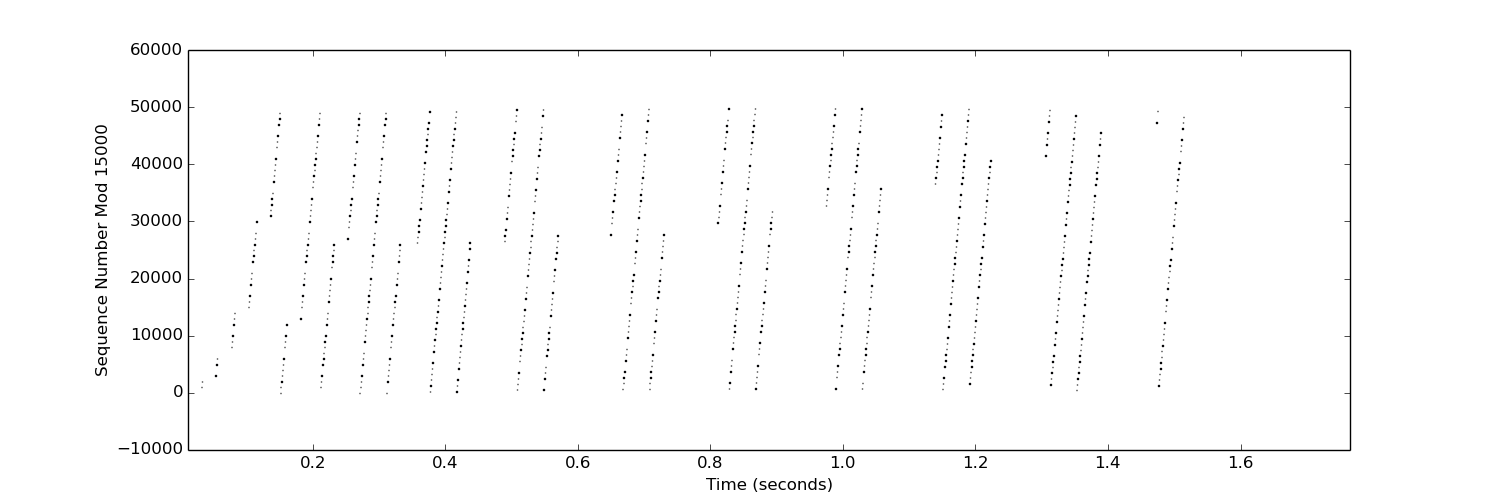
\includegraphics[width=17cm]{outputs/AIMD/AIMD_sequence1000.png}

\centerline{\emph{Figure 5.1a: Sequence Graph of the First of Two Flows in AIMD Mode}}

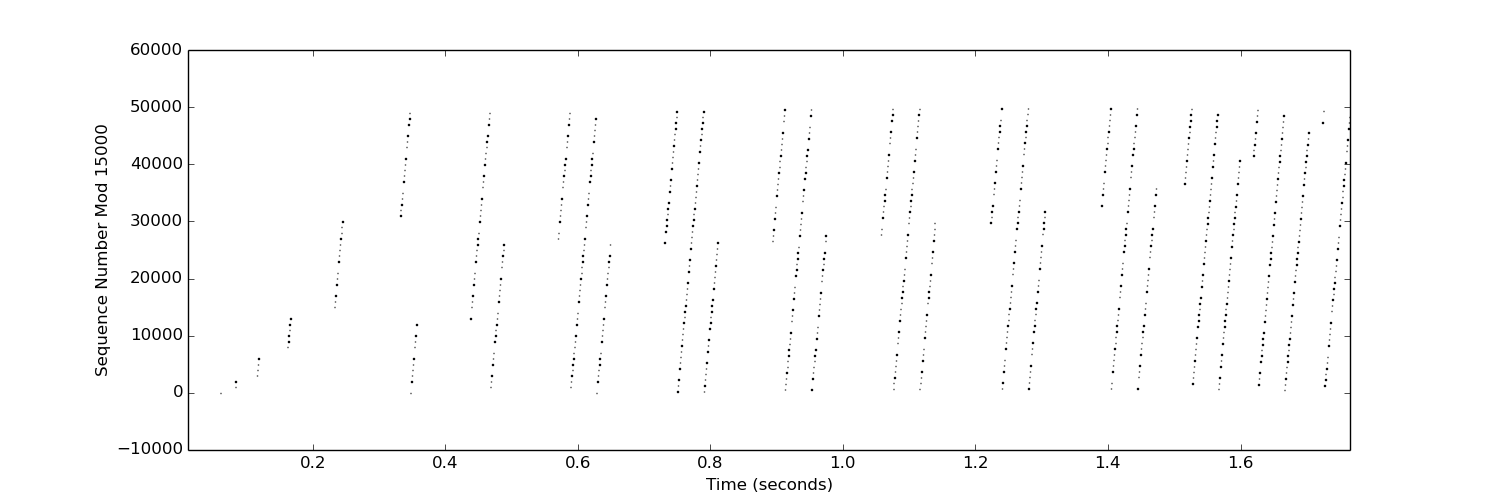
\includegraphics[width=17cm]{outputs/AIMD/AIMD_sequence2000.png}

\centerline{\emph{Figure 5.1b: Sequence Graph of the Second of Two Flows in AIMD Mode}}


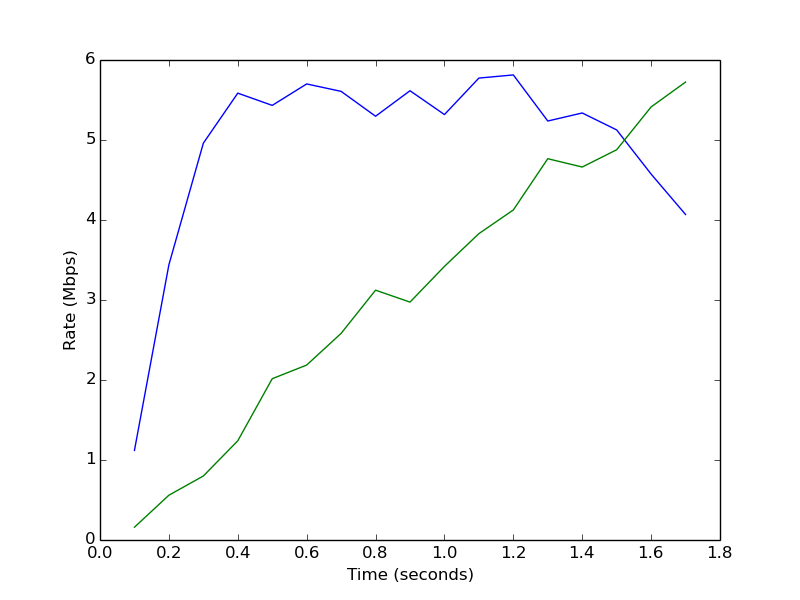
\includegraphics[width=17cm]{outputs/AIMD/AIMD_rate.png}

\centerline{\emph{Figure 5.2: Rate Graph of Two Flows in AIMD Mode}}

The first flow puts a large amount of segments on the line very rapidly, getting a jump start on the second flow. The second flow is increasing where it can, and is allowed a higher portion of the link when compared to AIAD (figure 4.2). 

If the second flow had been delayed even longer, and the first flow had to transfer a file larger than 1 MB, the graph would be more interesting. The blue line would be extremely close to 10 Mbps to start, but as time continued to pass, the blue line would share more and more of the link. If allowed to transfer long enough, they would both eventually reach 5 Mbps transfer speed.


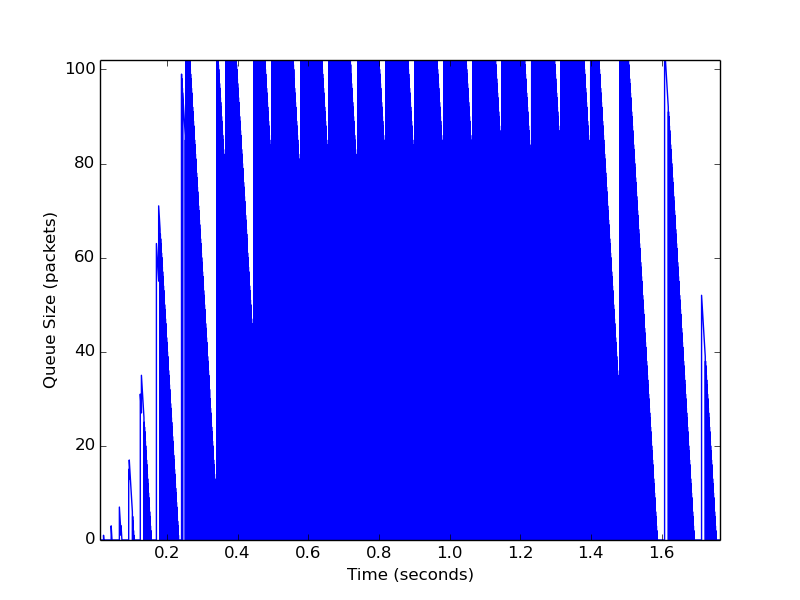
\includegraphics[width=17cm]{outputs/AIMD/AIMD_queue.png}

\centerline{\emph{Figure 5.3: Queue Graph of Two Flows in AIMD Mode.}}

The queue graph again shows that the queue is nearly full for nearly the entire duration.



% \vspace{5mm}
% \begin{absolutelynopagebreak}
% \begin{lstlisting}
% def loss_event(self):
%     self.threshold = max(self.window/2, self.mss)
%     self.window = 1 * self.mss

% # slow start & AI
% def increase_window(self, amount):
%     # loss event check
%     self.duplicates += 1
%     if amount == 0 and self.duplicates >= 4:
%         self.loss_event()
%     else:
%         self.duplicates = 0

%         # AI
%         if amount + self.window >= self.threshold:
%             self.window += (self.mss * amount / self.window)
%             self.threshold = self.window
%         # slow start
%         else:
%             self.window += amount
% \end{lstlisting}
% \end{absolutelynopagebreak}
% \vspace{5mm}

% \section{Tests}

% Slow Start: To test slow start, I transferred a small file that transferred entirely within the range of slow start. In the following graph, the reader should notice that each set of segments doubles in size. 

% 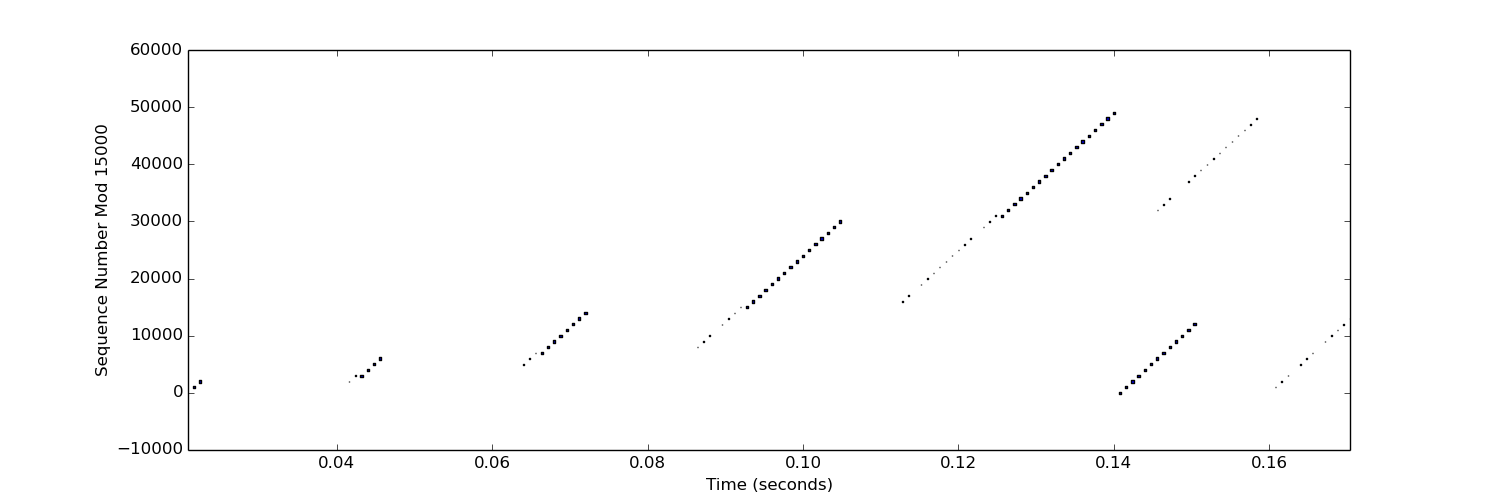
\includegraphics[width=17cm]{outputs/converted_output1.png}

% Additive Increase: To test additive increase, I transferred a larger file with a threshold of 16,000 bytes, i.e., 16 segments.  The reader can observe in the following graph that each set of segments doubles in size, like in the previous graph, until the sender sends 16 segments. The next set is 17 segments in size, and the final set is also 17 segments in size, which concluded the file transfer.

% 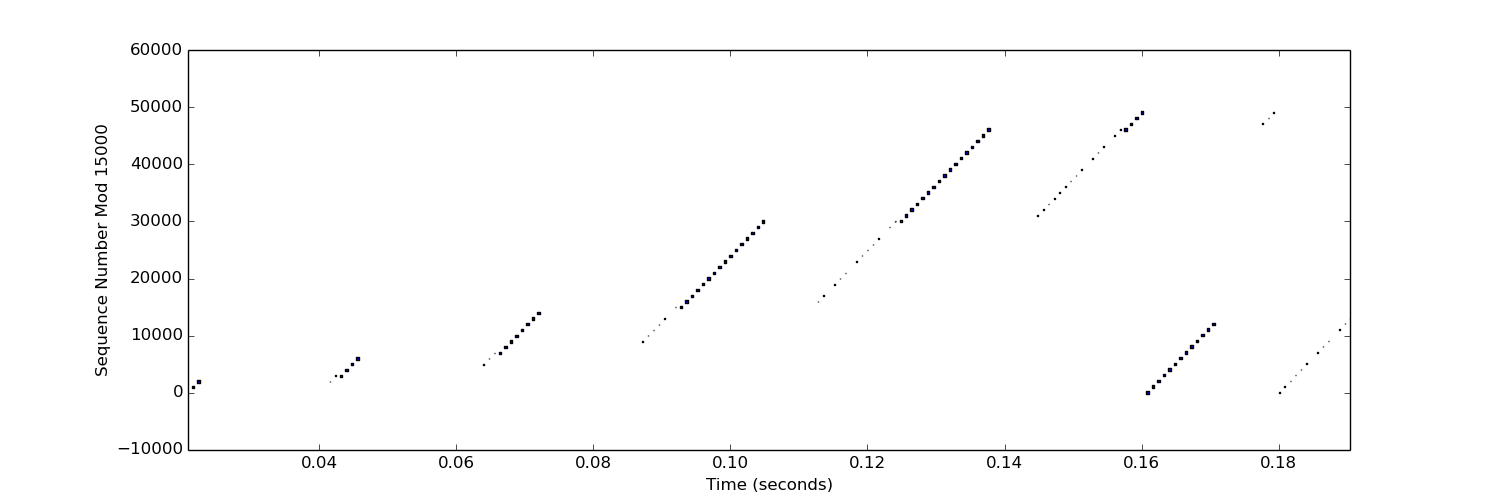
\includegraphics[width=17cm]{outputs/converted_output2.png}

\end{document}
